\documentclass{article}
\usepackage{graphicx} % Required for inserting images
\usepackage{amsmath}
\usepackage{geometry}
\usepackage{amssymb}
\usepackage{color}
\usepackage{CJKutf8}
\usepackage{float}
\usepackage{subfigure}
\usepackage{listings}
\usepackage{placeins}
\usepackage{enumitem}
\geometry{a4paper, scale=0.8}   
\linespread{2}
\definecolor{dark_green}{RGB}{0,102,51}
\title{Lab1 - Intro to Wireshark}
\author{Jiaxi Zhang}
\date{\today}
\begin{document}
\maketitle
\begin{CJK*}{UTF8}{gbsn}

\section{Three Different Protocols}
\begin{itemize}
    \item \textbf{HTTP} : Hypertext Transfer Protocol. It is from the application layer of the OSI model. It is used
    to transfer hypertext and display it on the web browser between the client and the server.
    \item \textbf{ARP} : Address Resolution Protocol. It is from the link layer of the OSI model. It is used to map
    an IP address to a MAC address so that the data can be correctly transmitted in LAN.
    \item \textbf{TCP} : Transmission Control Protocol. It is from the transport layer of the OSI model. It is used
    to establish a reliable data transmission between two hosts.
\end{itemize}

\section{Analysis for Packets 76-85}
The application protocol used in the packets 76-85 is HTTP which
can be seen in packet 79 and 82 in the Protocol column, and in the Info
column, we can see the GET request in 79 and the HTTP/1.1 200 OK response in 82.
The total time for the request and response is 0.007246 seconds,
which can be computed by the time difference between packet 79 and 82
(27.724984 - 27.717738 = 0.007246 seconds). The screenshot of the
third question is shown below.
% include image
\begin{figure}[H]
    \centering
    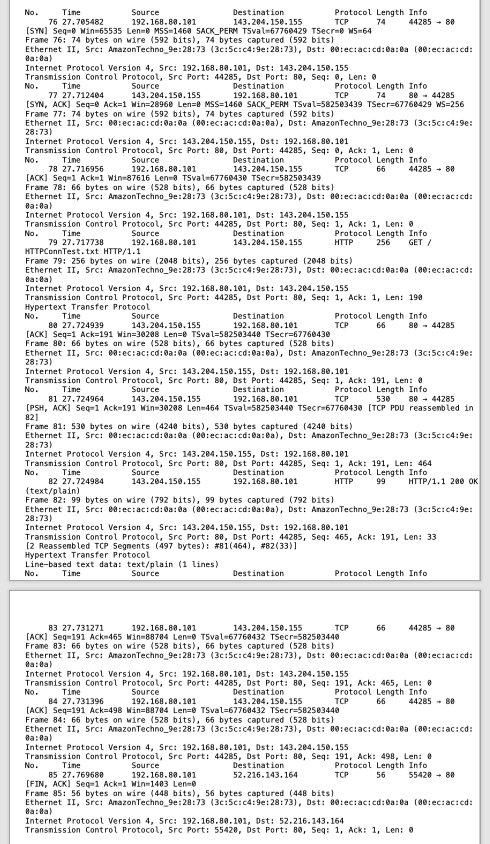
\includegraphics[width=0.8\textwidth]{Q3.png}
    \caption{Packets 76-85}
\end{figure}

\section{Analysis for Packets 89-91}
\subsection{}
Packets 89-91 does not contain any application layer protocol because
TCP requires connection establishment before data transmission. In this case,
packets 89-91 are used to establish the connection between the client and the server
with 3 handshake steps. Then we can find in packet 92 that the application layer
protocol is HTTP with is a GET request,
which also indicates the connection has been established successfully
in the previous 3 packets.

\subsection{The closure of this connection}
Packet 226 and 227 are correlated with the closure of this connection mentioned above.
It can be seen by tracking the sequence number 9 in the filter bar. In packet 226, the
server sends a FIN flag to the client to request the closure of the connection.
Then in packet 227, the client sends an ACK flag to the server to acknowledge the
request.

\end{CJK*}
\end{document}
